\documentclass[tikz,border=10pt]{standalone}
\usepackage{tikz}
\usetikzlibrary{angles,quotes,animations}

\begin{document}

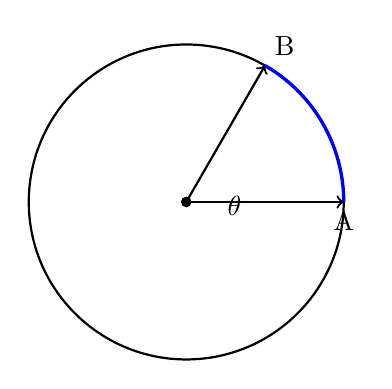
\begin{tikzpicture}[scale=2]
    % Draw the circle
    \draw[thick] (0,0) circle (1);
    
    % Mark the center
    \filldraw[black] (0,0) circle (0.03);
    
    % Draw the radius
    \draw[thick,->] (0,0) -- (1,0) coordinate (A);
    
    % Draw an arc for the angle
    \draw[thick,->] (0,0) -- ({cos(60)},{sin(60)}) coordinate (B);
    
    % Draw the arc with an animation
    \draw[domain=0:60,samples=50,smooth,variable=\t,very thick,blue] 
         plot ({cos(\t)},{sin(\t)});
    
    % Label the angle
    \node[below right] at (0.2,0.1) {$\theta$};
    
    % Add the points A and B
    \node[below] at (1,0) {A};
    \node[above right] at ({cos(60)},{sin(60)}) {B};
\end{tikzpicture}

\end{document}
